\documentclass[12pt,oneside,notitlepage,abstracton,a4paper]{article}
\usepackage{epsfig,scrpage2,graphicx}
\usepackage[
	separate-uncertainty=true,
	per-mode=symbol-or-fraction,
]{siunitx}
\usepackage[
	textwidth=3cm
]{todonotes}
\usepackage{amsmath}
\setcounter{secnumdepth}{3}

\setlength{\parindent}{0em}
\setlength{\parskip}{0ex plus0.5ex minus0ex}
\pagestyle{scrheadings}
\bibliographystyle{unsrt}   

\renewcommand{\headfont}{\normalfont}


\title{\Large Thermal Performance of the Petal Prototype} 
\author{\normalsize Anja Beck, TU Dortmund, Germany \\[3ex]
DESY Summer Student Programme 2018 \\[3ex]
ATLAS Experiment}
\date{\normalsize \today}

\begin{document}
	\makeatletter
	\begin{titlepage}
		\begin{center}
			\ \\[10ex]
			{\huge \bfseries  \@title }\\[10ex] 
			{\LARGE  \@author}\\[10ex]
			{\large \@date}\\[30ex] 
			
\includegraphics[width=0.3\linewidth]{img/DESY_logo_4C.eps}\hspace{20ex}
			
\includegraphics[width=0.3\linewidth]{img/ATLAS-Logo-Square-Blue-RGB.eps}
		\end{center}
	\end{titlepage}
	\makeatother
	\thispagestyle{empty}
	\newpage
	\setcounter{page}{1}

\begin{abstract}

\noindent
\end{abstract}

\newpage

\tableofcontents
\newpage 

\section{Introduction}
The high-luminosity upgrade for the LHC planned to be ready to run in 2026 imposes new challenges on detectors. For instance, an enhanced luminosity is immediately related to elevated radiation levels which constitute heat development. To avoid a thermal runaway and ensure reliable measurements, the electronics must be held at a constant temperature\todo{How cold should it be?}\ which requires some kind of cooling system for all detector components.

\subsection{Petal}
The summer student project documented in this report was related to the thermal performance tests of the inner tracking detector of the ATLAS experiment. Figure \ref{fig:ATLAS} illustrates its position within the big detector and the planned upgraded design. The parts studied at DESY are the so-called petals that are assembled perpendicularly around the beampipe to track particles with low transversal energy. Figure \ref{fig:petal} displays a picture of the tested petal prototype.
\begin{figure}[h!]
	\centering
	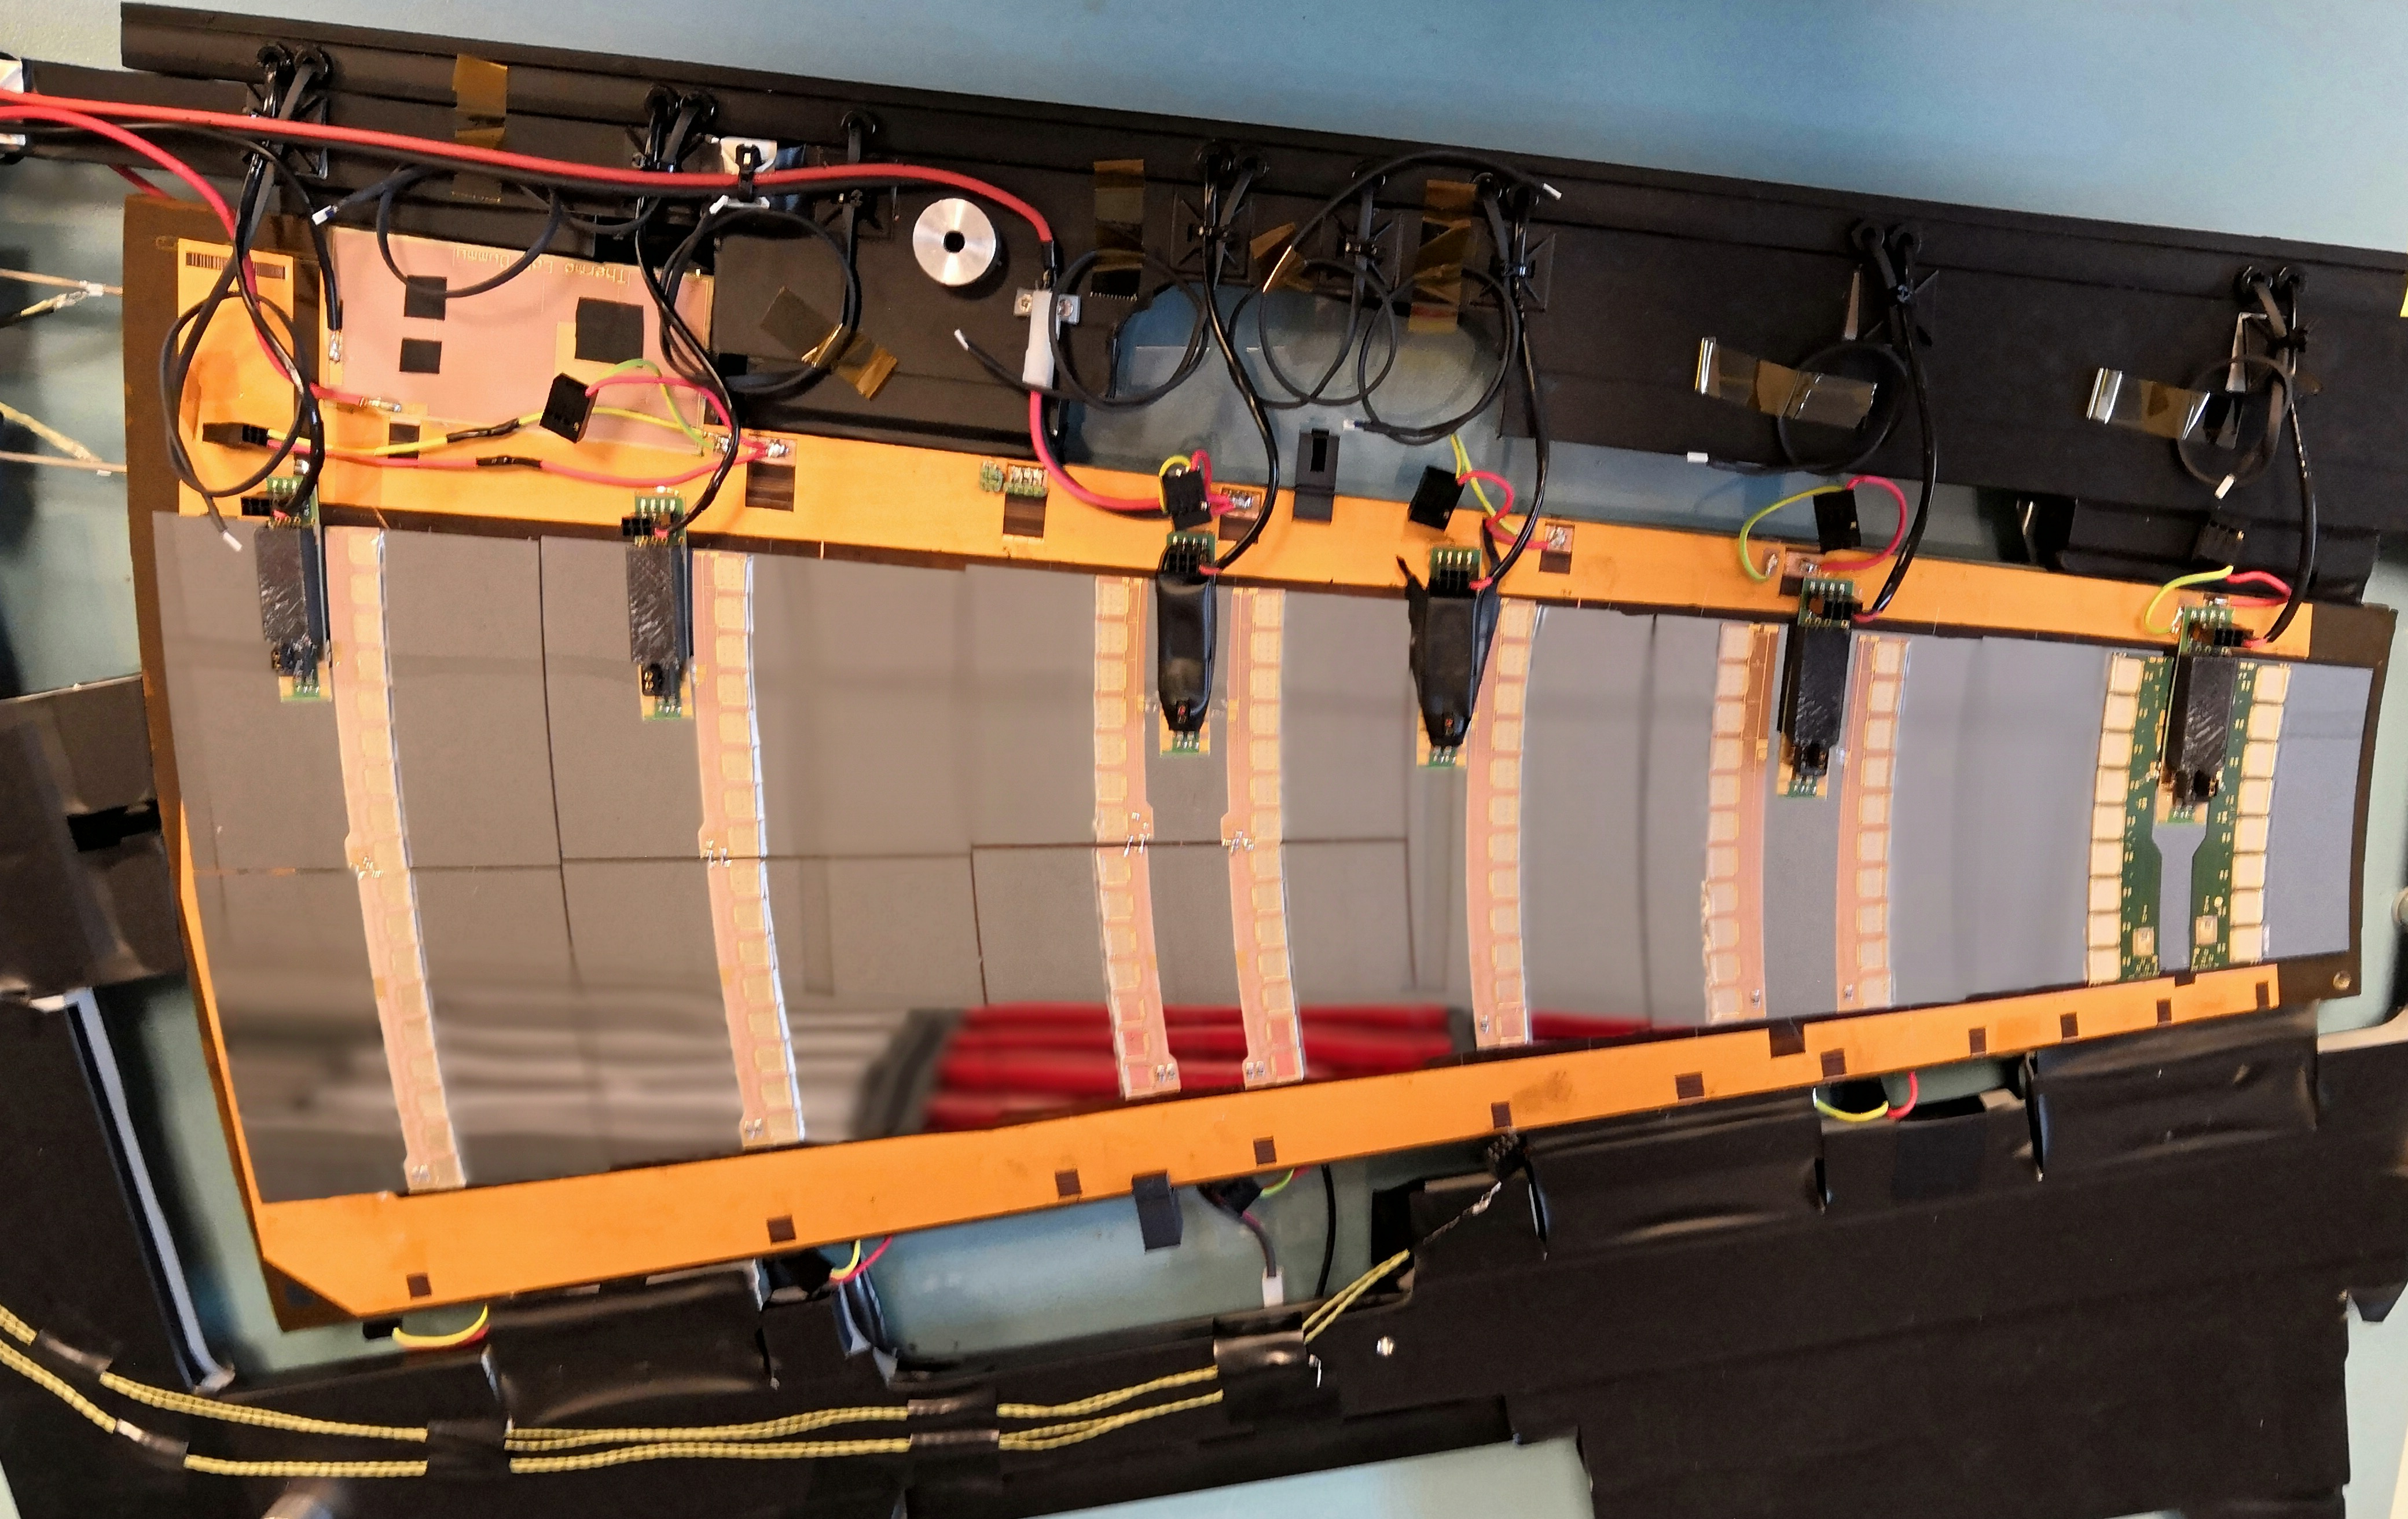
\includegraphics[width=.6\textwidth]{img/petal.jpg}
	\caption{Picture of the tested petal prototype.}
	\label{fig:petal}
\end{figure}
\subsection{Cooling System}
Figure \ref{fig:coolingLoop} shows a prototype of the bare cooling loop. The cooling system is based on the energy needed for a phase change. Liquid $\text{CO}_2$ is pumped into the cooling loop where some of it evaporates if exposed to heat. This evaporation requires energy (enthalpy of evaporation) which is taken from the heat source.
\begin{figure}[h!]
	\centering
	\tikz[baseline=(a.north)]\node[yscale=-1,inner sep=0,outer sep=0](a){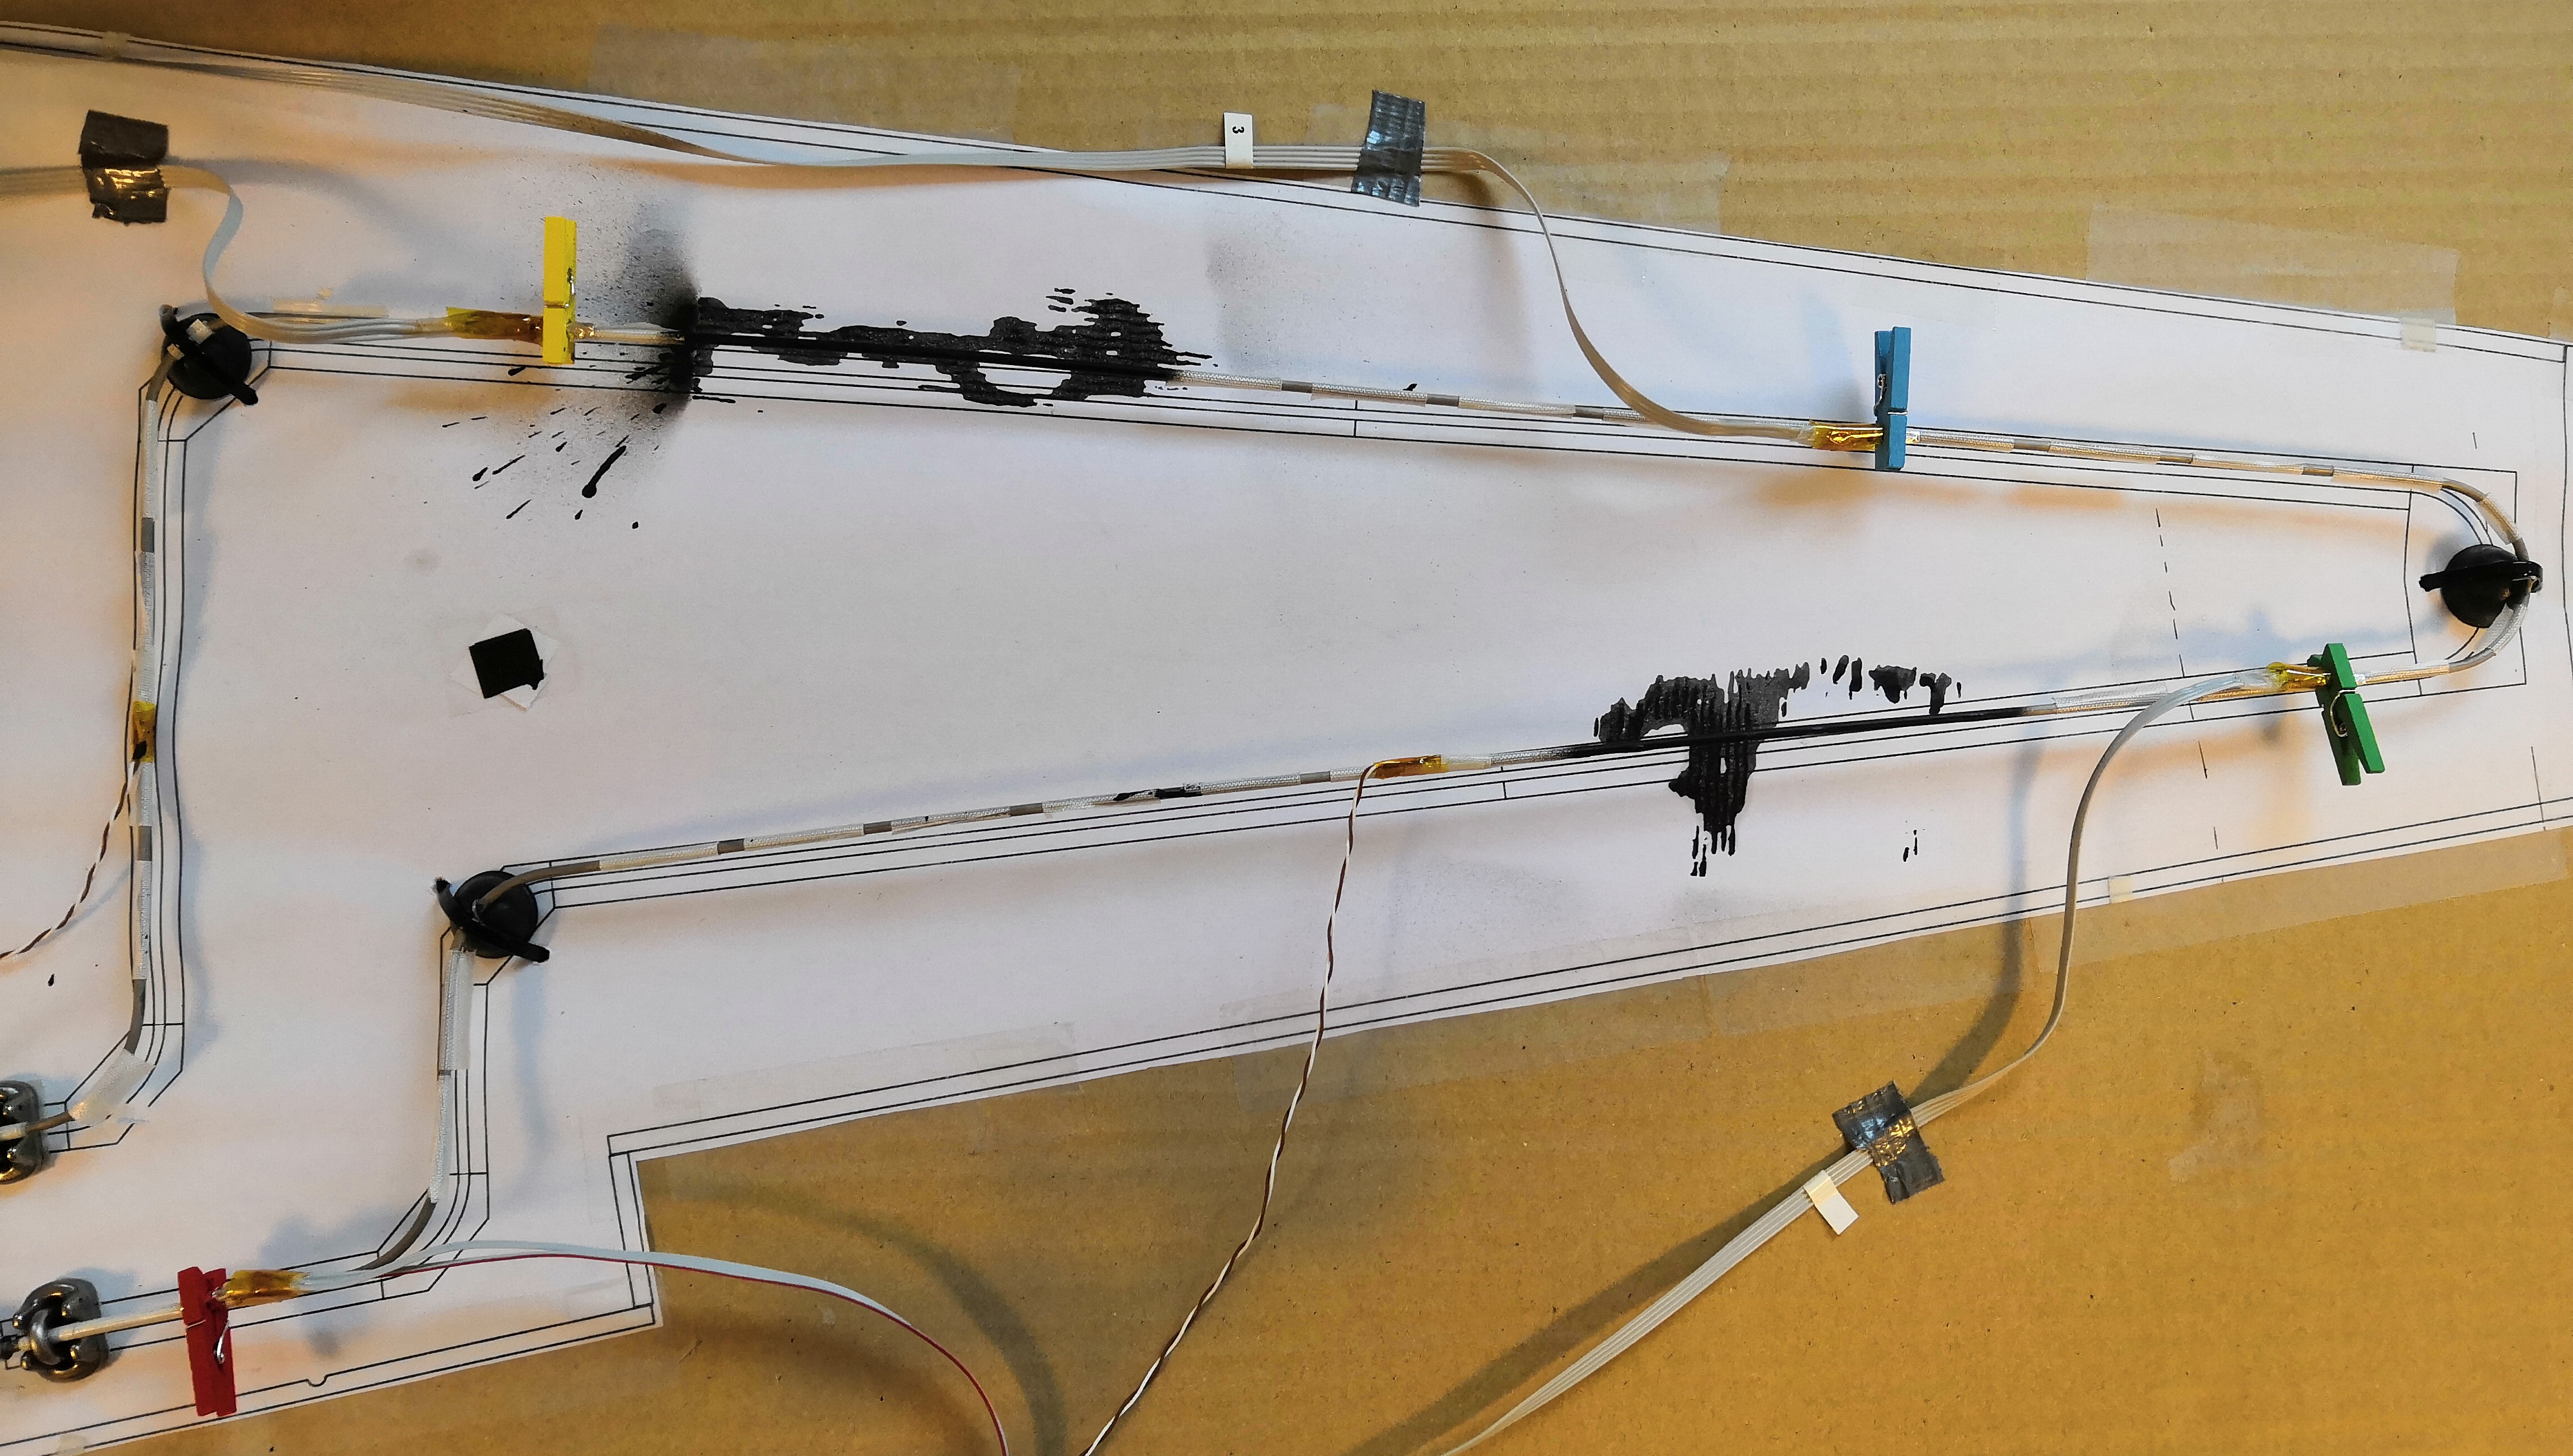
\includegraphics[width=.6\textwidth]{img/coolingLoop.jpg}};
	\caption{Picture of the a bare cooling loop.}
	\label{fig:coolingLoop}
\end{figure}

\begin{landscape}
\begin{figure}[h!]
	\centering
	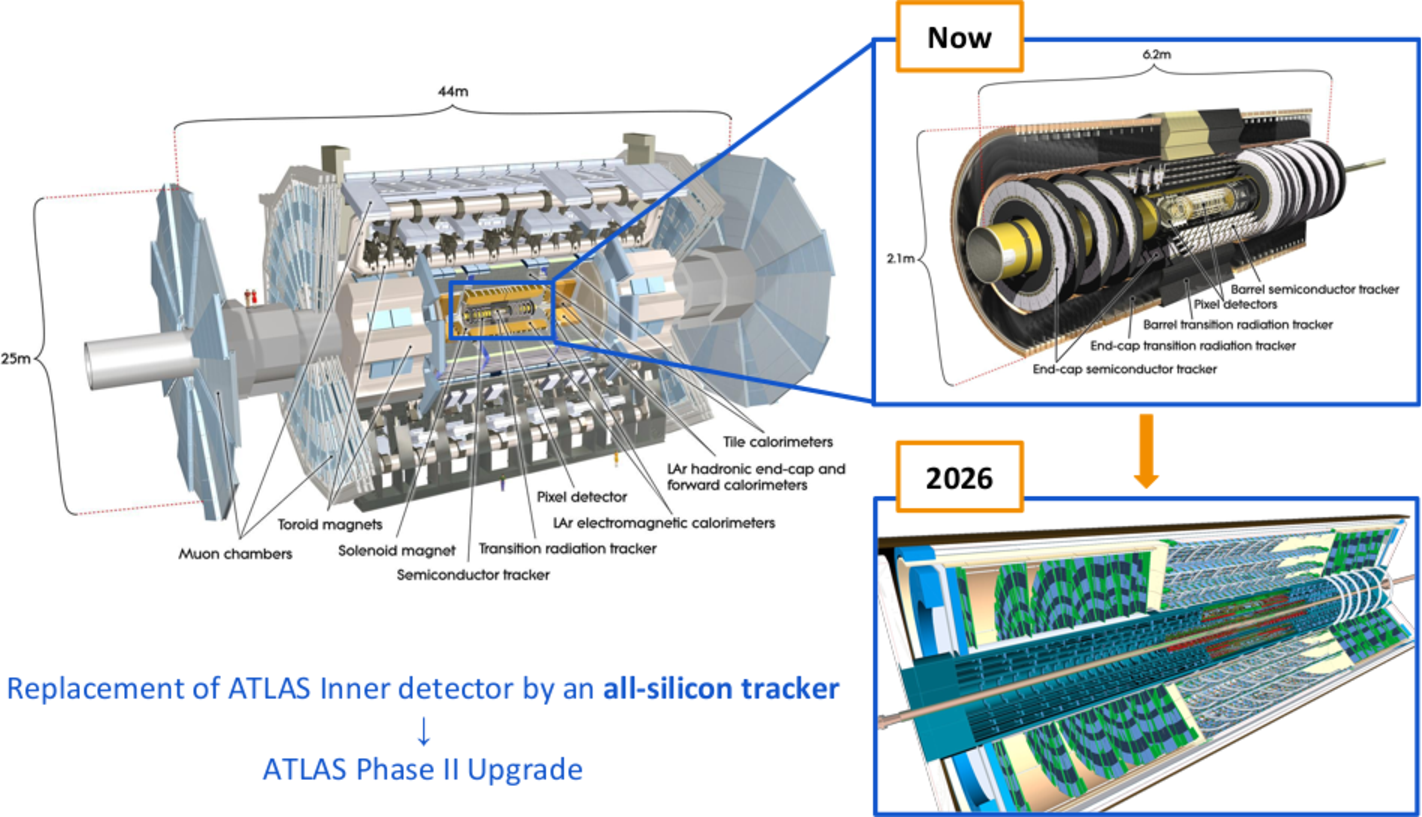
\includegraphics[height=0.9\textwidth]{img/ATLAS.pdf}
	\caption{Schematics of the upgrade of the ATLAS inner tracking detector.}
	\label{fig:ATLAS}
\end{figure}
\end{landscape}

\section{IR}
To assess the thermal performance of the petal, we measure the emitted radiation in the infrared (IR) spectrum. To properly evaluate the data measured with the IR camera, we need to understand the behaviour of IR radiation and camera software. This section gives an overview over these topics.
\subsection{Emissivity}
Every body emits IR radiation depending on its temperature. Light in the IR spectrum behaves identical to the more intuitive visible light. This means that surfaces can emit, absorb, and reflect IR radiation. Being purely interested in the \textit{emitted} power, we need to minimize reflection in the IR region. The emissivity $\epsilon$ describes the ability of a surface to reflect IR radiation. \todo{Is it really only IR or is there an emissivity for all ranges?} It is a value between $0$ and $1$, where $0$ corresponds to total reflection, whereas $1$ corresponds to no reflection. So, to achieve good results using IR measurements, we cover the petal with a high emissivity coating. The determination of the exact emissivity value for the chosen paint is described in section \ref{sec:emissivityMeasurement}.

\subsection{Software}

\subsection{Theory}
To fully comprehend and also for being able to check the camera data, a theoretical relation between the emitted power and temperature is crucial. As we are trying to approach an ideal black body using the high emissivity paint, Planck's law for black body radiation,
\begin{align}
	p(\lambda, T) = \frac{2hc^2}{\lambda^5}\frac{1}{\exp\left(hc/(\lambda k_\text{B}T)\right)-1} \ ,
\end{align}
can be a good start. \todo{Describe variables!} The IR camera measures radiation over a range of wavelengths, so we need to integrate this and obtain
\begin{align}
	P(T) = \int_{\lambda_\text{min}}^{\lambda_\text{max}}\frac{C_1}{\lambda^5}\frac{1}{\exp\left(C_2/(\lambda T)\right)-1}\ \text{d}\lambda \ .
\end{align}
Taking account of reflections of the ambiance, we propose the following equation
\begin{align}
	P_\text{tot.}(T) = \underbrace{\epsilon P(T)}_\text{emission} + \underbrace{(1-\epsilon)P(T_\text{amb.})}_\text{reflection of ambiance} \ .
\end{align}\todo{Describe variables!}

\clearpage

\section{Emissivity Measurements\label{sec:emissivityMeasurement}}


\section{Tests on the Petal}
\subsection{Preparations}
% Glue tests, Gluing, Paint tests, Painting
\subsection{First Results}

\section{More}
% Describe all the smaller things I did? Liveplotting, etc.?


\clearpage
\begin{thebibliography}{99}
\begin{sloppypar}
\bibitem{my_reference} Study of ...
{\em Author name}
\end{sloppypar}
\end{thebibliography}

\end{document}
